\documentclass[a4paper,listof=totoc,toc=sectionentrywithdots,abstract=false]{scrartcl}
\usepackage[affil-it]{authblk}

\usepackage{graphicx}
\usepackage[ngerman,english]{babel}
\usepackage{textcmds}
\usepackage{float}
\usepackage{csquotes}
\usepackage{tabularx}
\usepackage{pifont}% http://ctan.org/pkg/pifont

\newcommand{\cmark}{\ding{51}}%
\newcommand{\xmark}{\ding{55}}%

\usepackage[
backend=biber,
%style=chicago-authordate,
%citestyle=chicago-authordate,
%style=numeric,
%citestyle=numeric,
%style=authoryear,
%citestyle=authoryear,
style=alphabetic,
citestyle=alphabetic,
maxnames=1,
maxalphanames=1,
]{biblatex}

\renewcommand*{\labelalphaothers}{}

\DefineBibliographyStrings{english}{%
	andothers = {\em et\addabbrvspace al\adddot}
}

\addbibresource{biblatex.bib} %Imports bibliography file
\usepackage[colorlinks=false,hidelinks]{hyperref}

%\titlefoot{\centering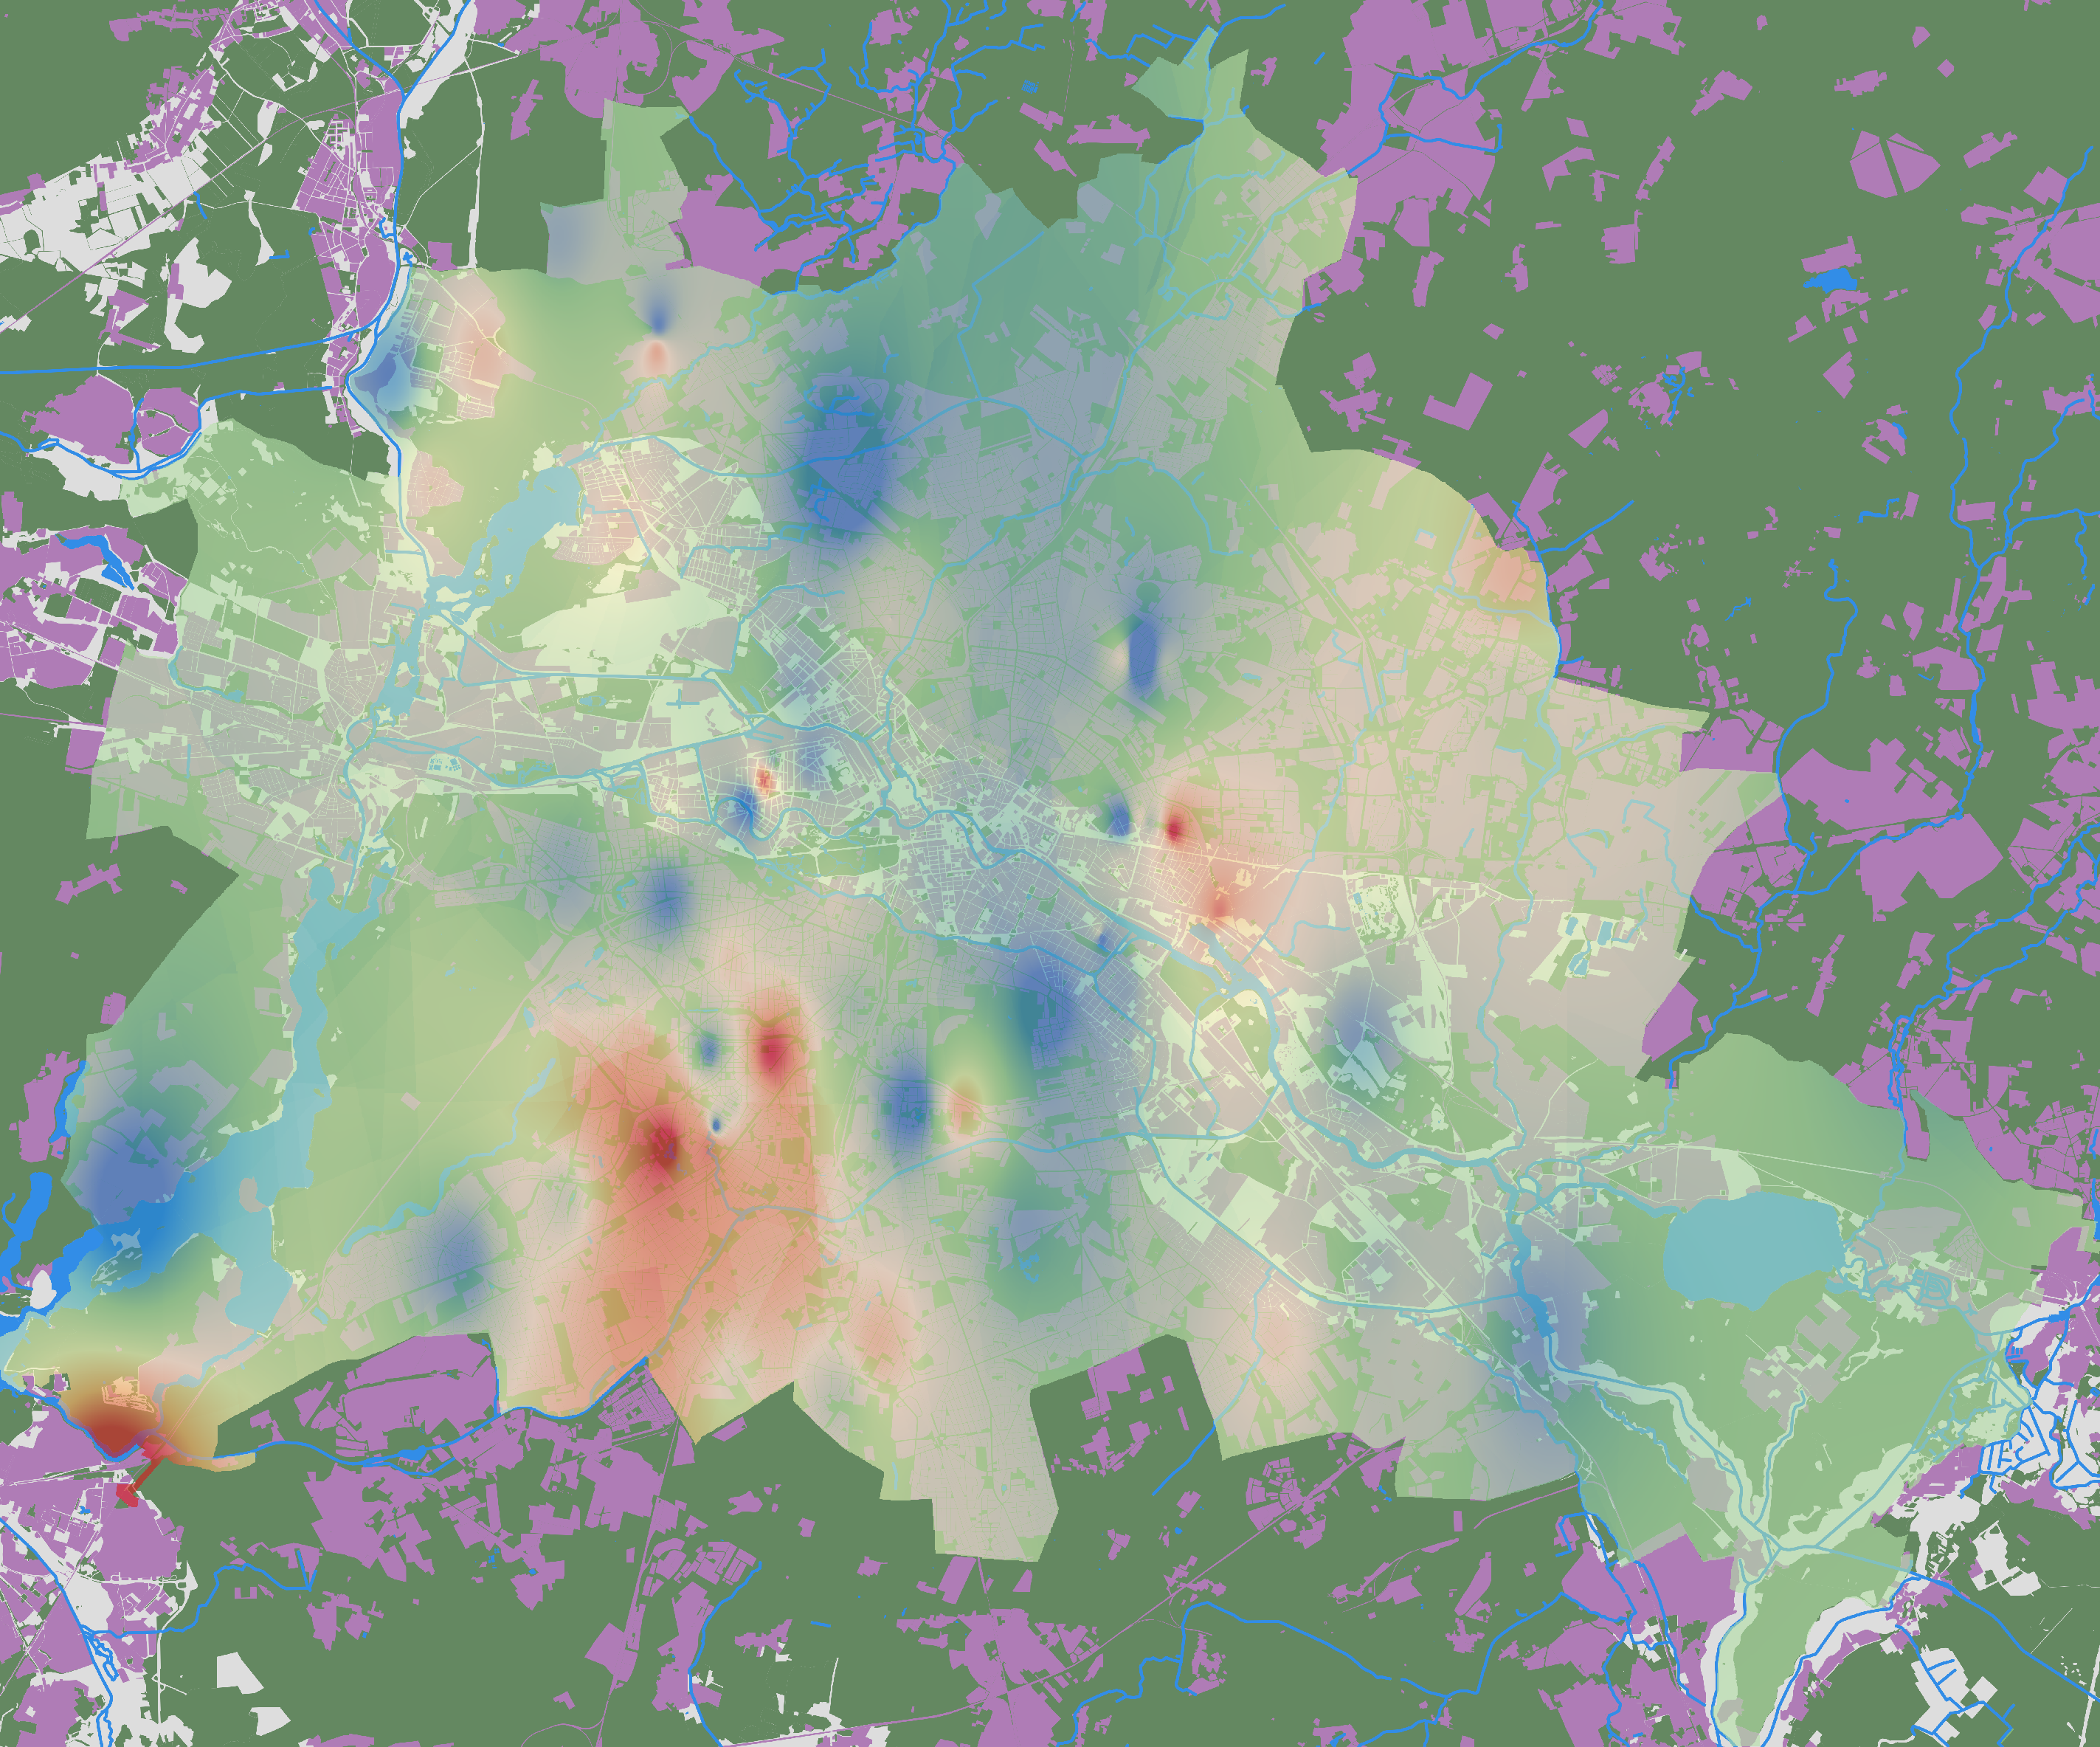
\includegraphics[width=6cm]{images/title}}
\title{Interpolation - Heat island effect on the example of Berlin}
\subtitle{FOSSGIS Seminar 2020}
\date{\today}
\author{Anja Doppelmayr \& Malte Heinzelmann}
\affil{Ruprecht-Karls-Universit\"at Heidelberg}
\graphicspath{images/}

\begin{document}

\maketitle

%{\centering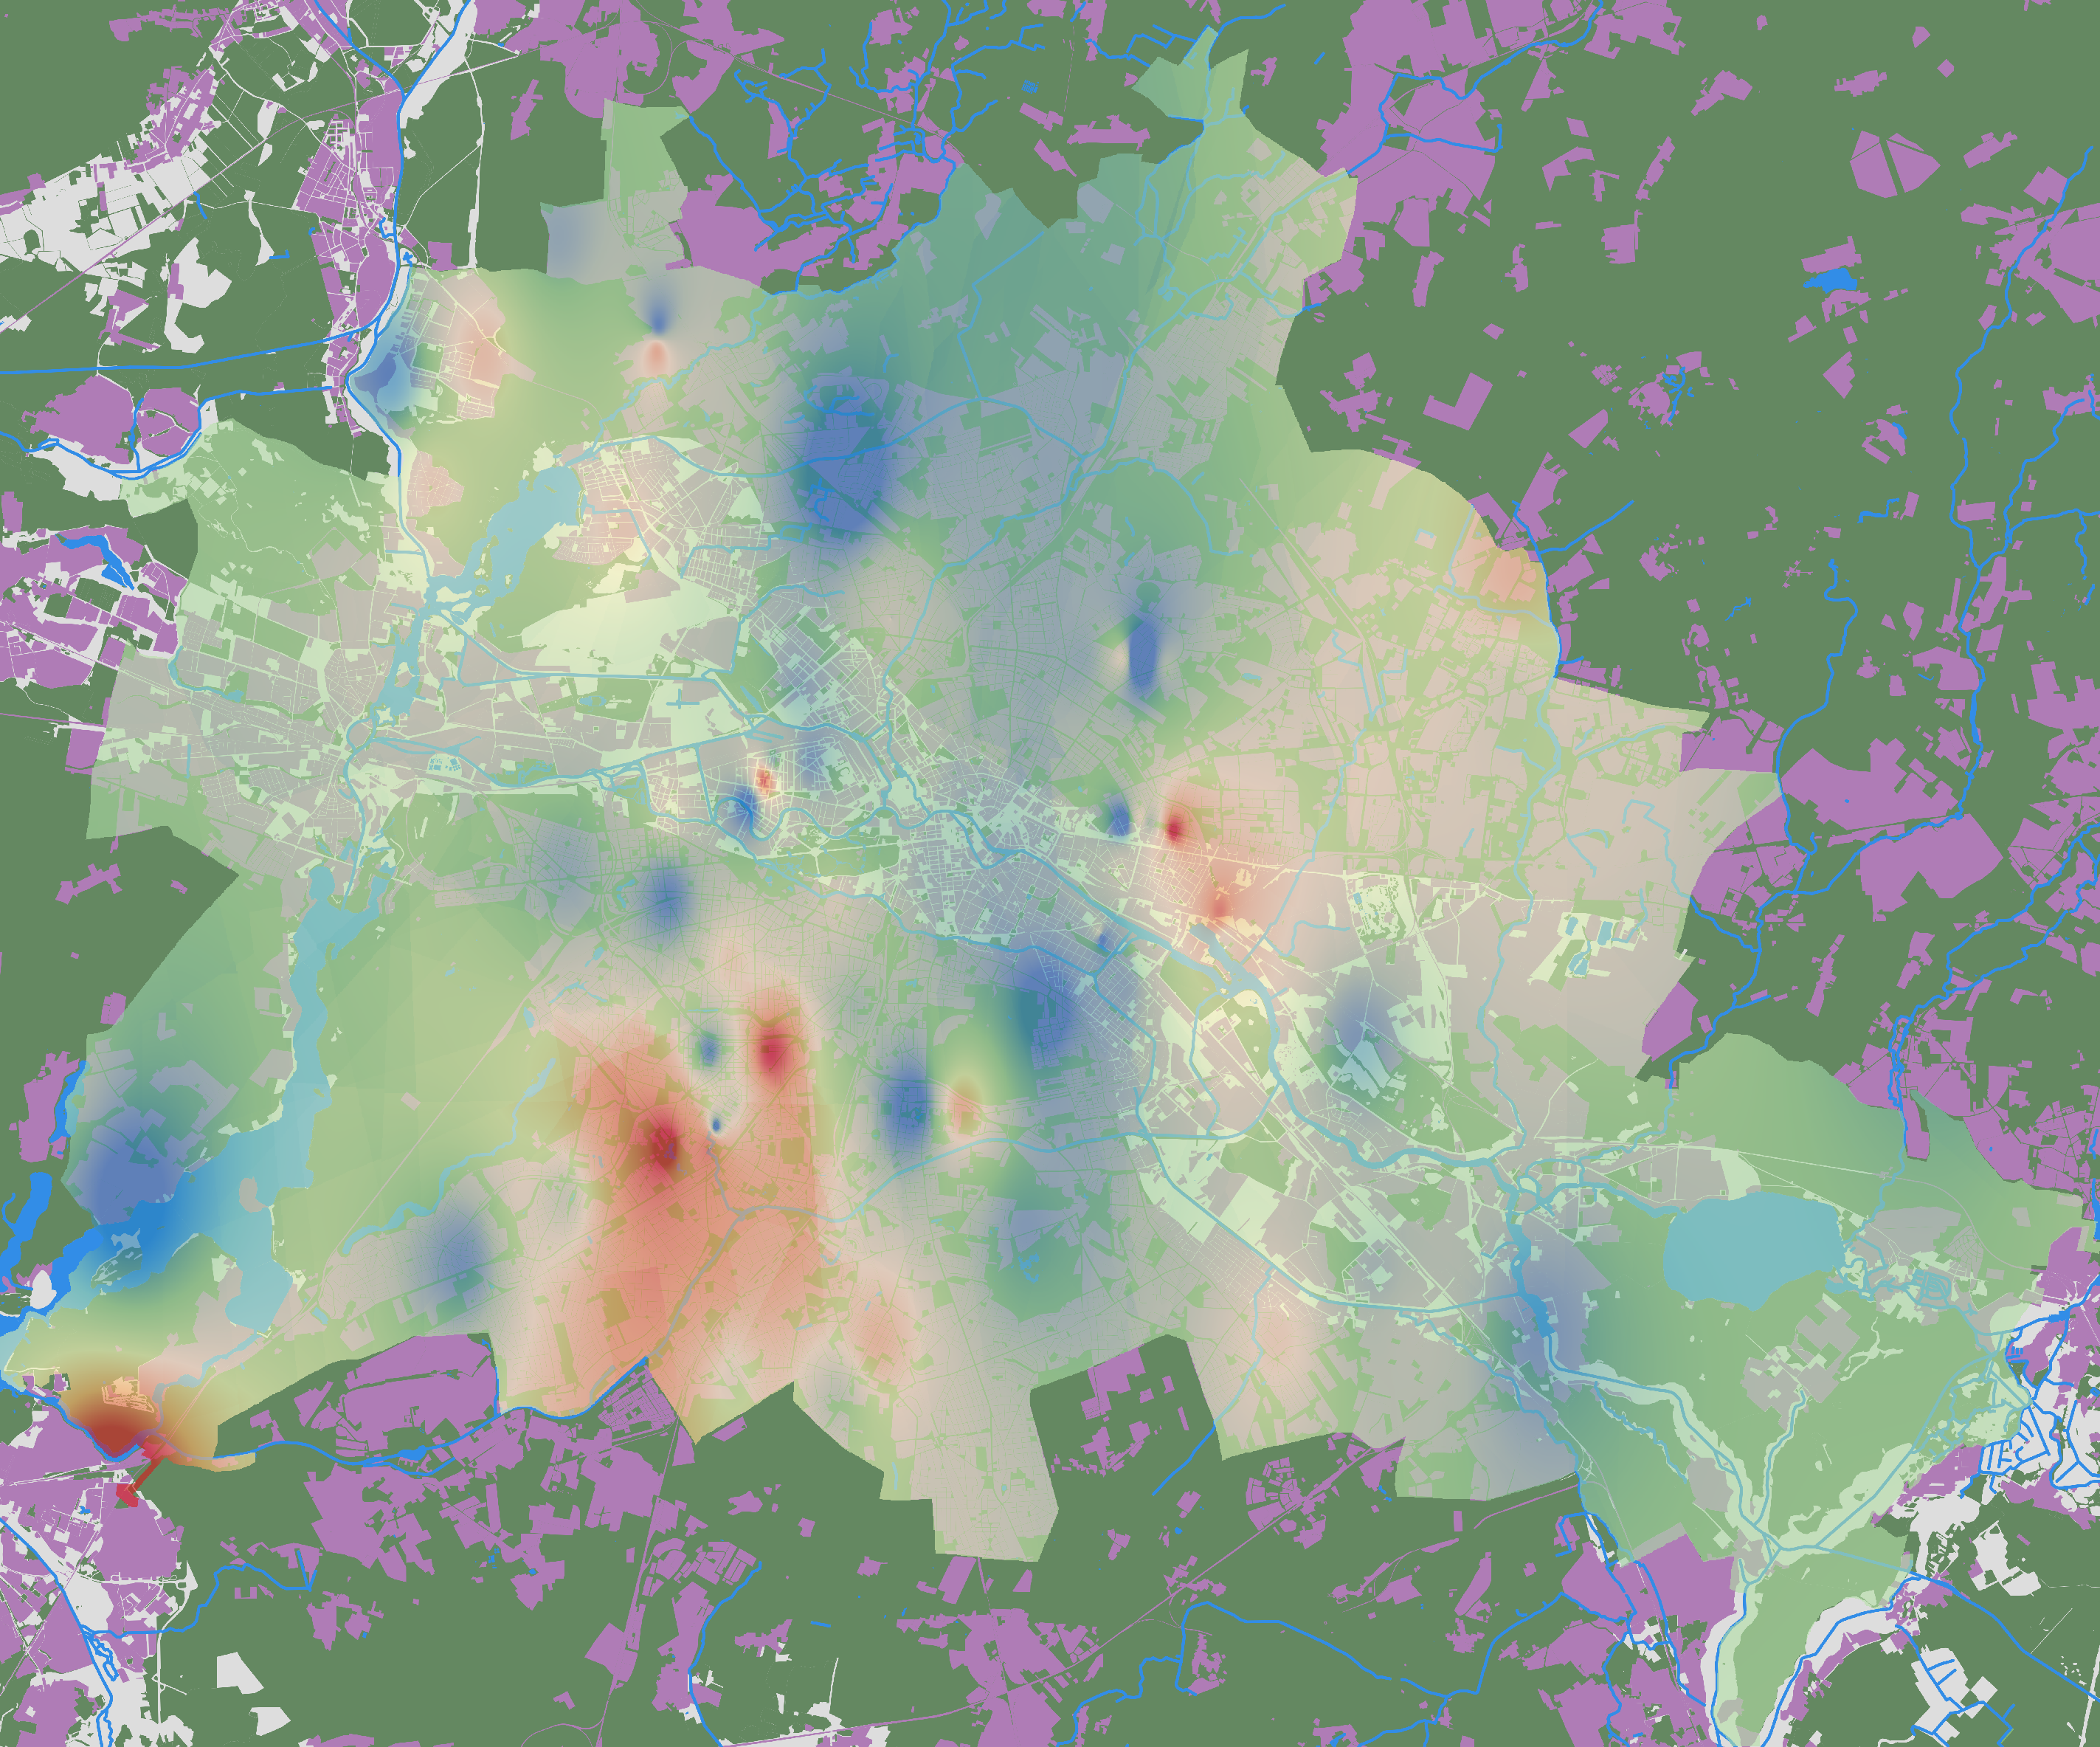
\includegraphics[width=6cm]{images/title}}

\begin{abstract}
	\setlength{\parindent}{0pt}
	% !TeX root = ../document.tex

TODO: Abstract
\end{abstract}

%\pagebreak
%\tableofcontents
%\pagebreak


% !TeX root = ../presentation.tex

\section{Introduction}
\begin{frame}{What is interpolation?}
	\begin{columns}[T] % align columns
		\begin{column}{.48\textwidth}
			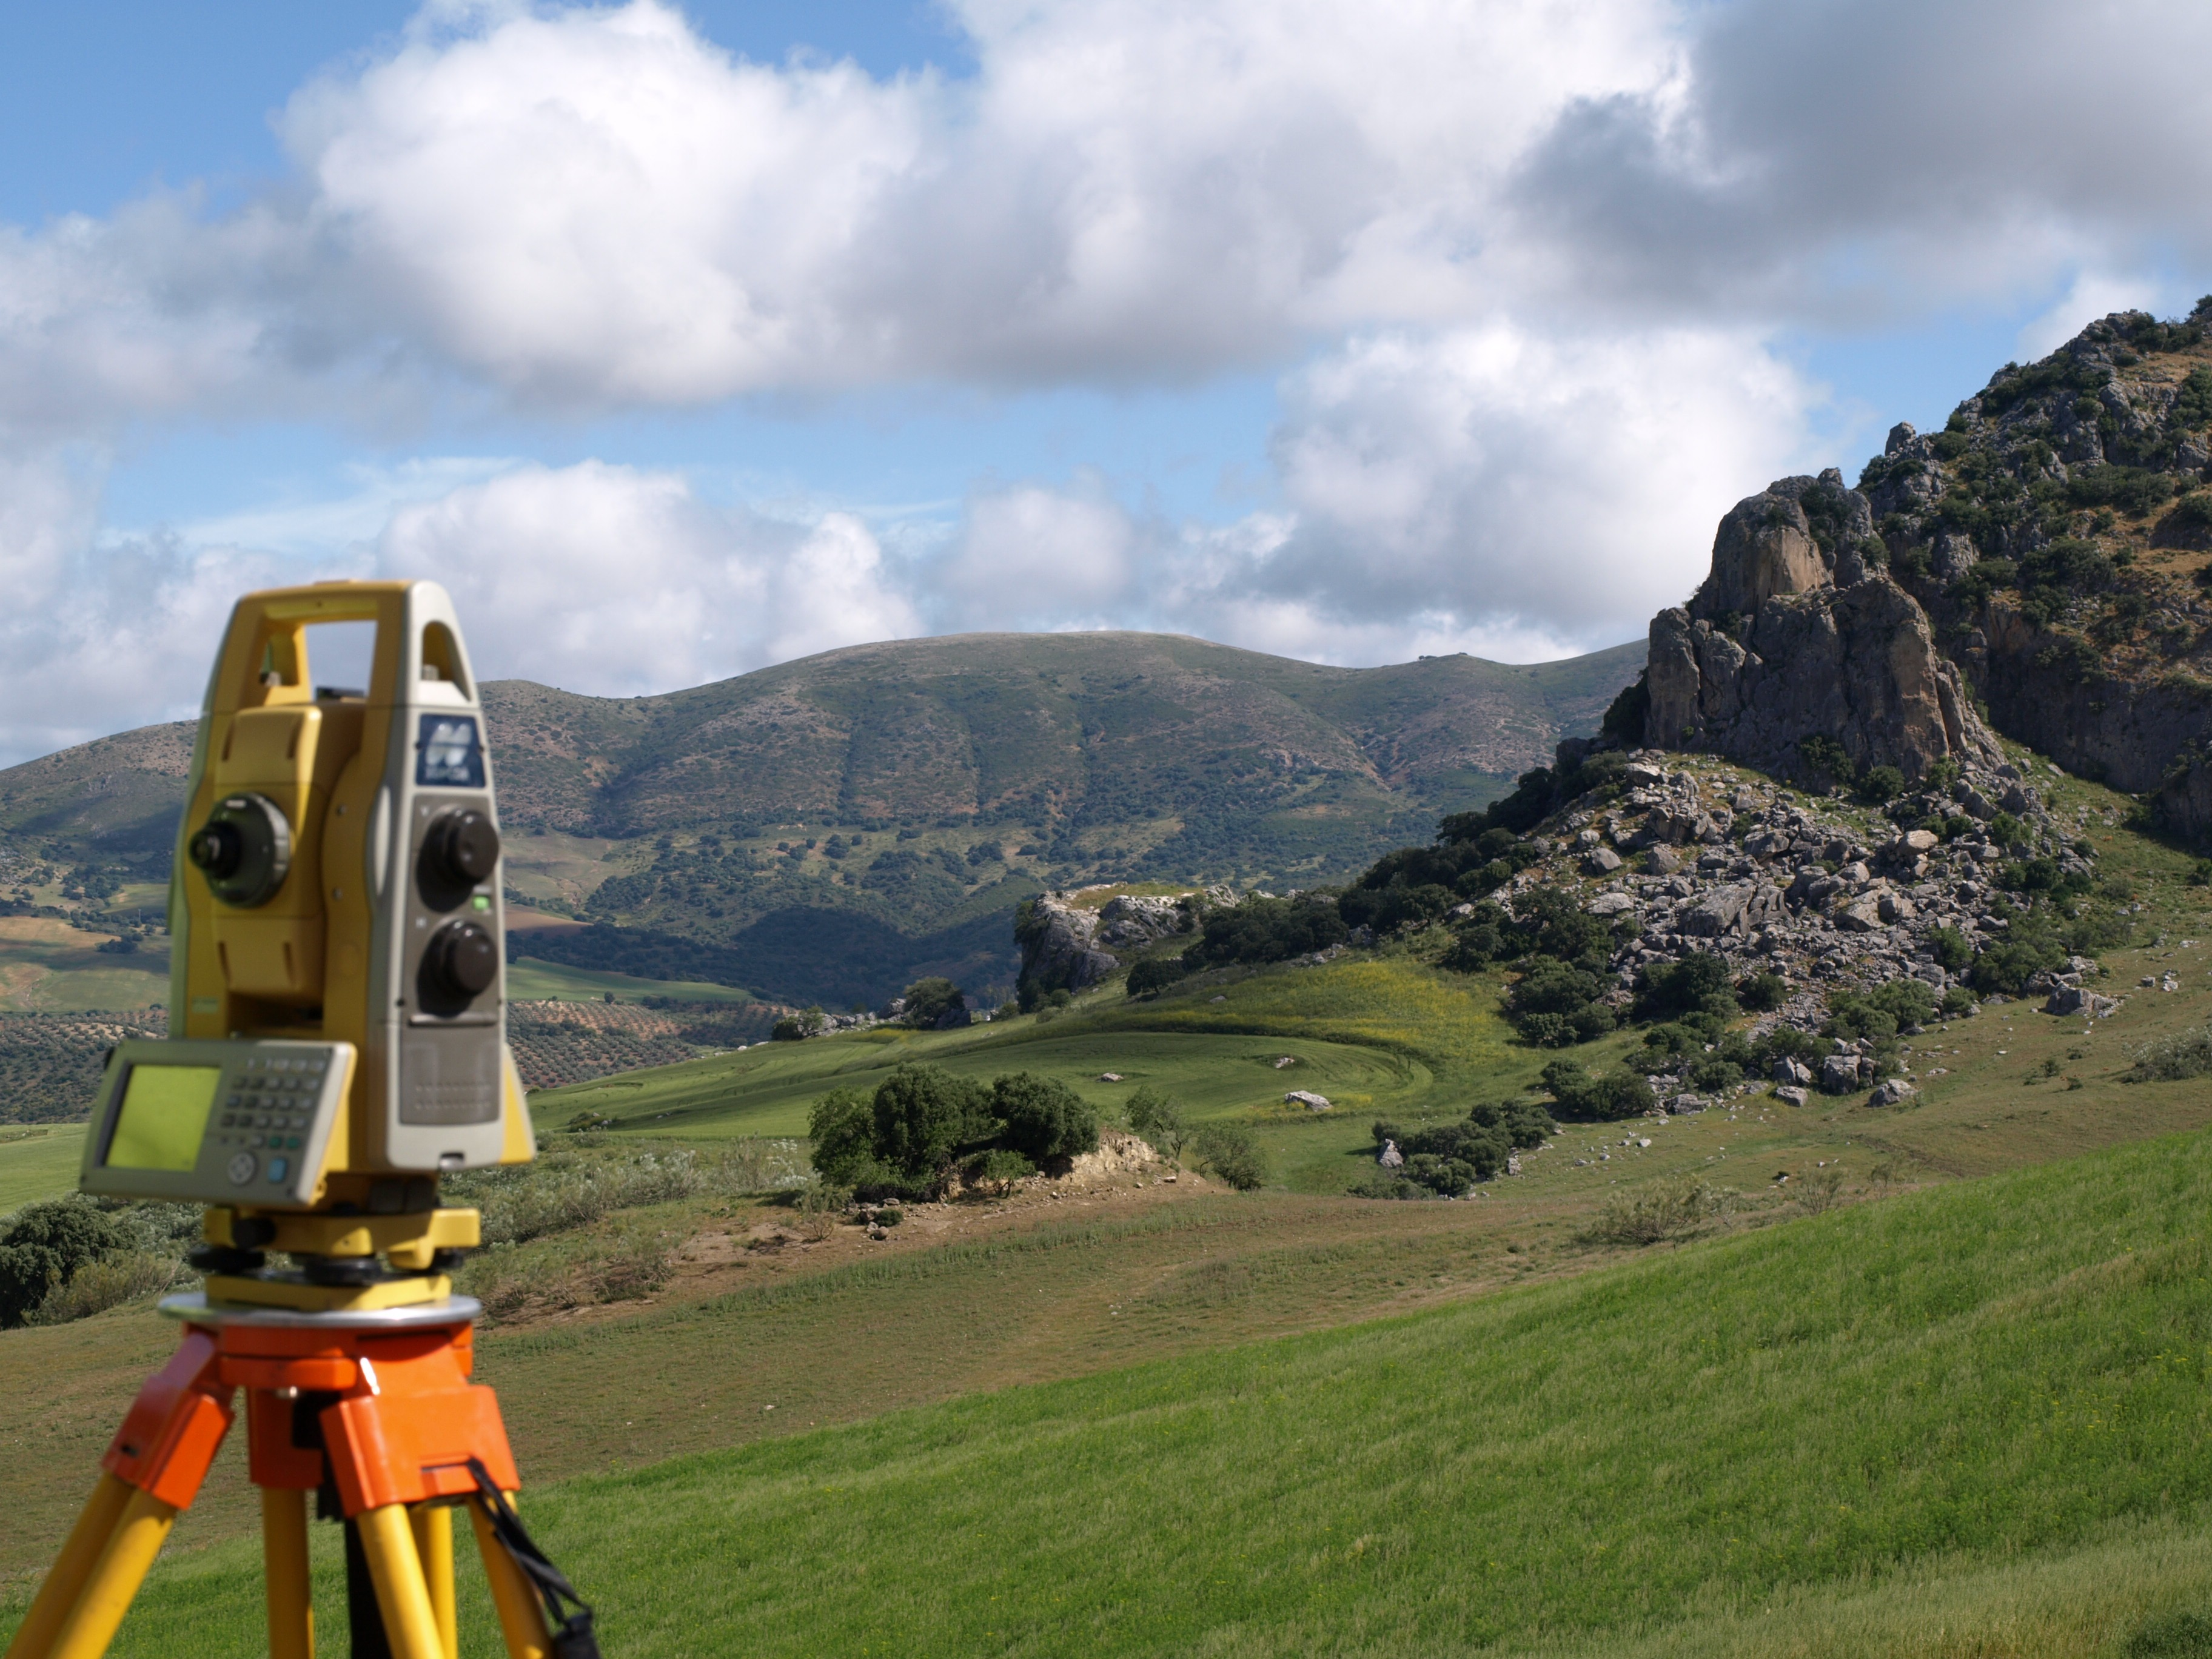
\includegraphics[width=\linewidth]{images/background}
		\end{column}%
		\hfill%
		\begin{column}{.56\textwidth}
			\begin{itemize}
				\item TODO
				\item TODO 2
			\end{itemize}
		\end{column}%
	\end{columns}
	\note{say "hello" now}
\end{frame}
\begin{frame}{This is interpolation!}
\begin{columns}[T] % align columns
	\begin{column}{.56\textwidth}
		\begin{itemize}
			\item TODO
		\end{itemize}
	\end{column}%
	\hfill%
	\begin{column}{.48\textwidth}
		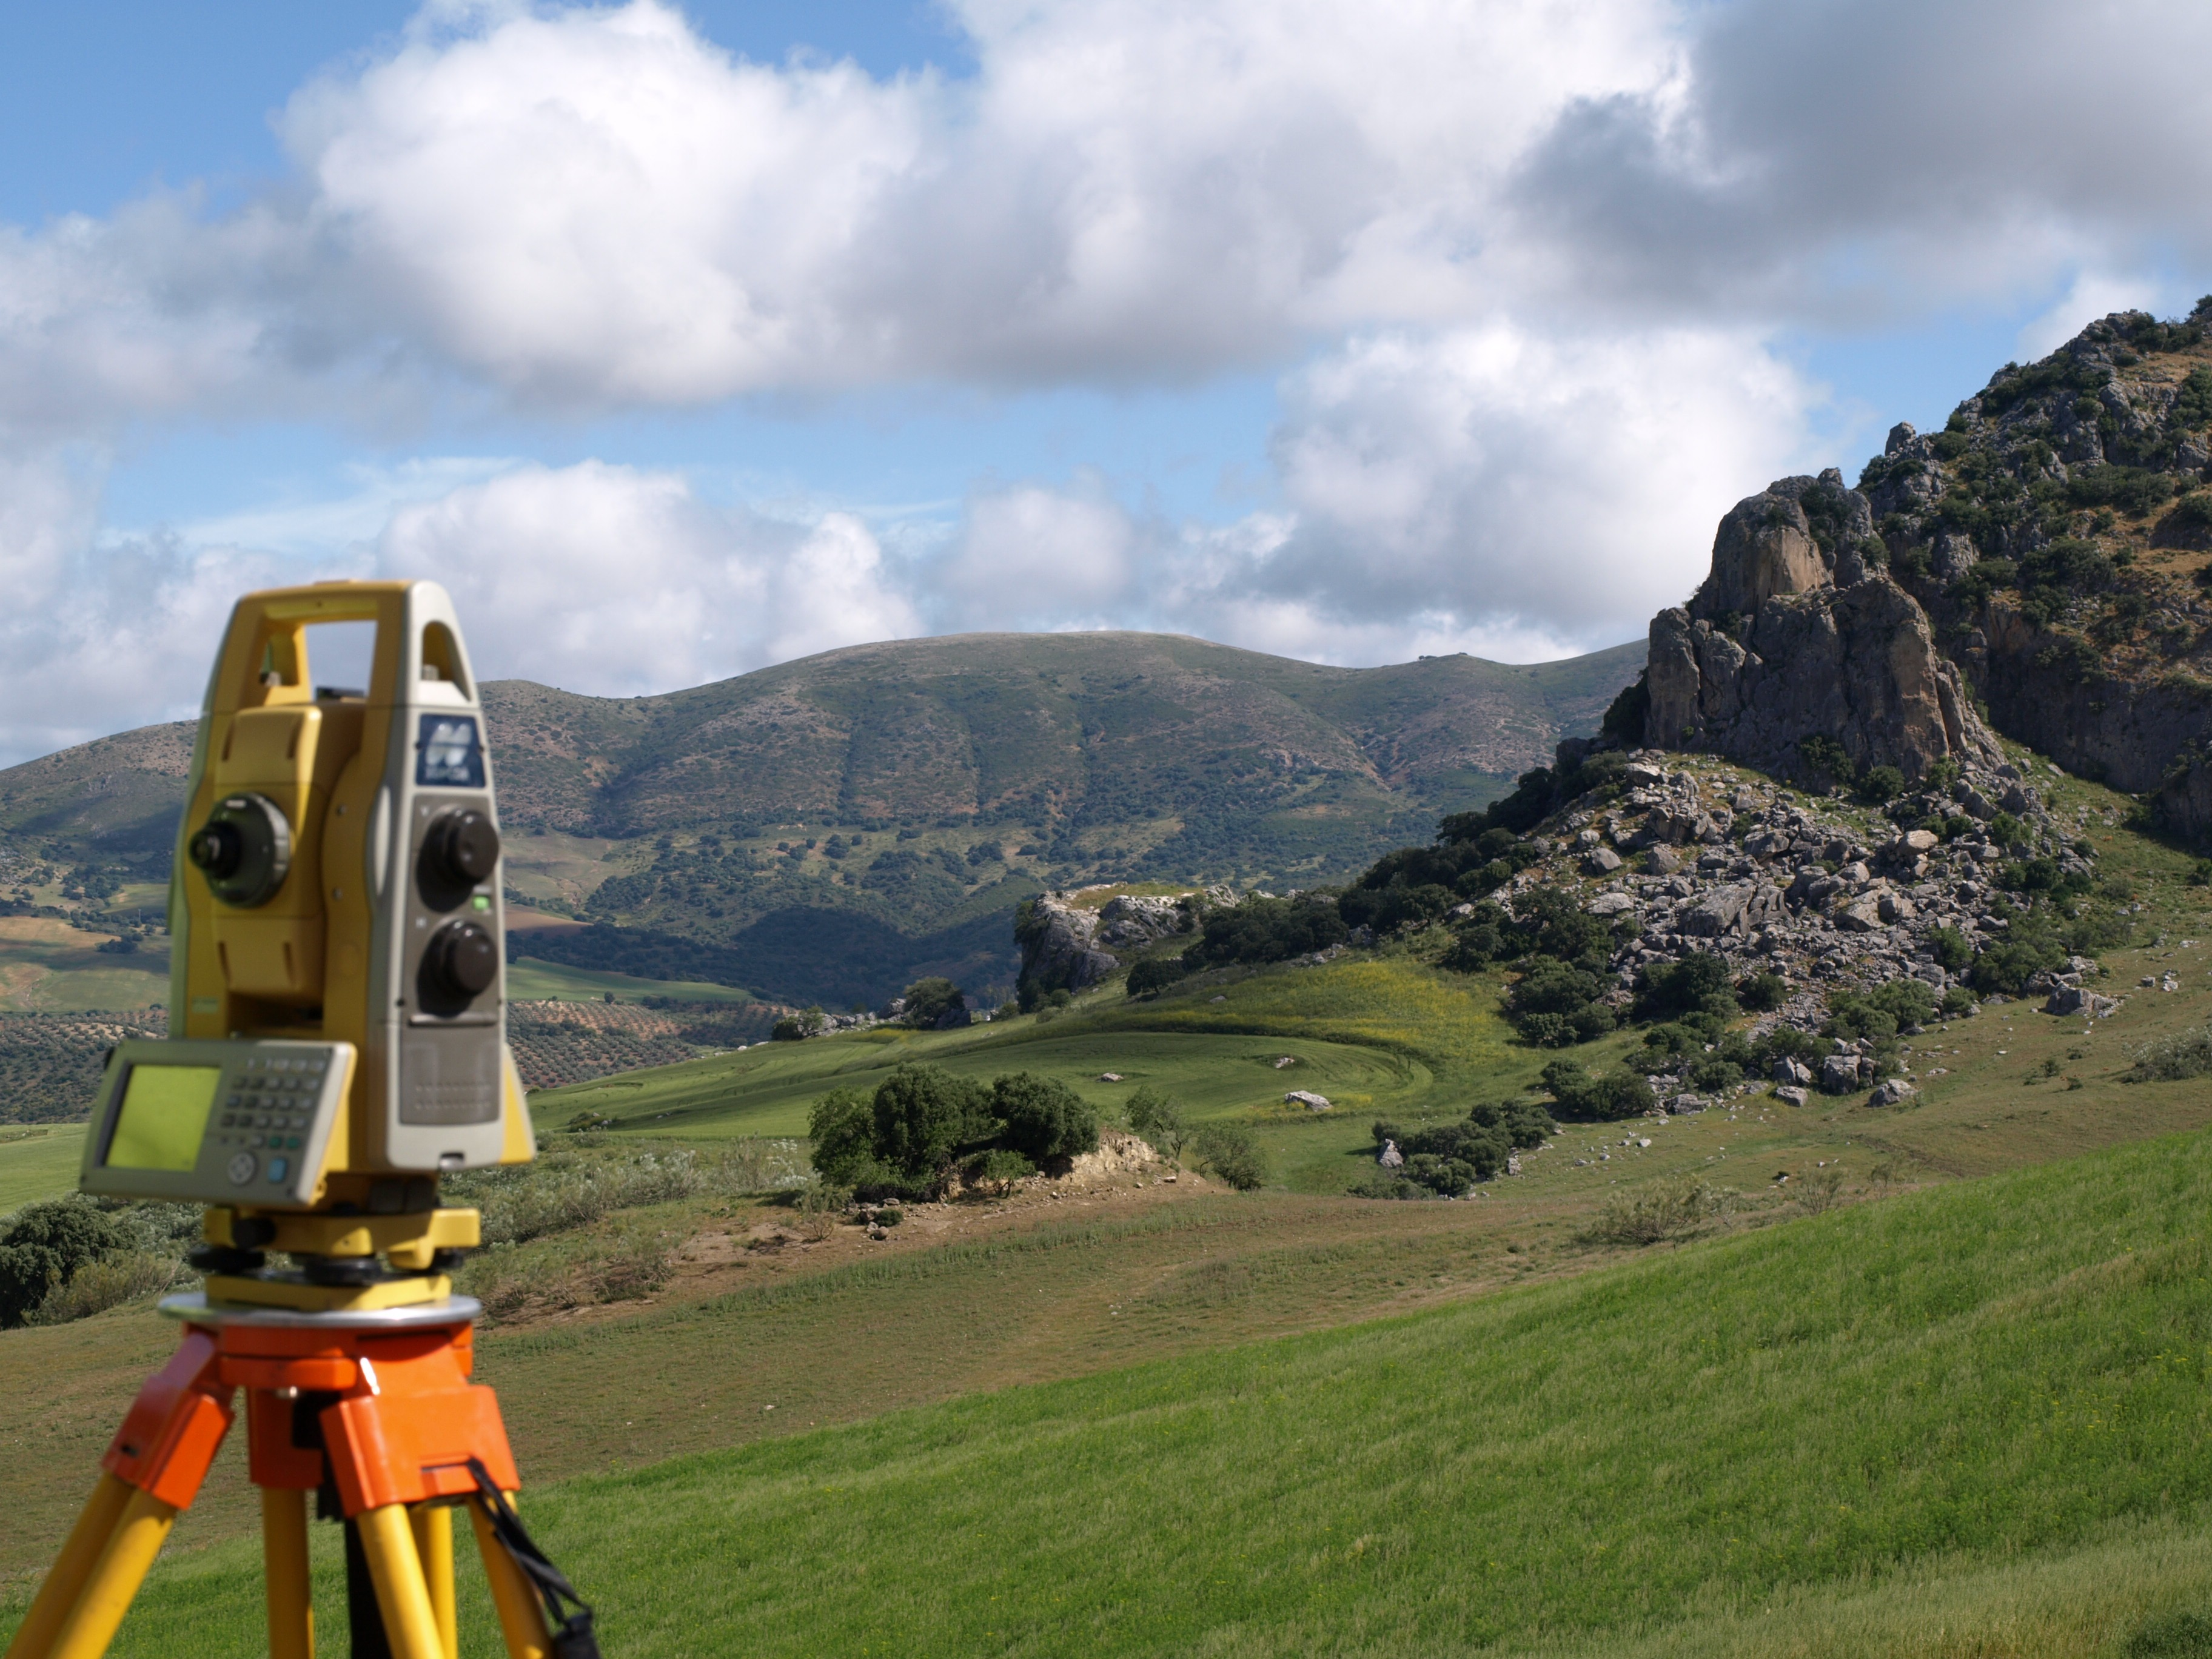
\includegraphics[width=\linewidth]{images/background}
	\end{column}%
\end{columns}
\note{say "hello" now}
\end{frame}
% !TeX root = ../document.tex

\section{Introduction}

The following chapter describes interpolation in general with regard to the most frequently used methods. We will give an introduction to the background of each method, their suitability/advantages and disadvantages as well as examples of application in other studies. Furthermore, we present possibilities of carrying out interpolation analysis and an overview of which methods are supported by a variety of FOSSGIS tools.

% TODO: difference deterministic/statistical methods

\subsection{}
% !TeX root = ../presentation.tex

\section{Results}
\begin{frame}{Results}
	\begin{columns}[T] % align columns
		\begin{column}{.48\textwidth}
			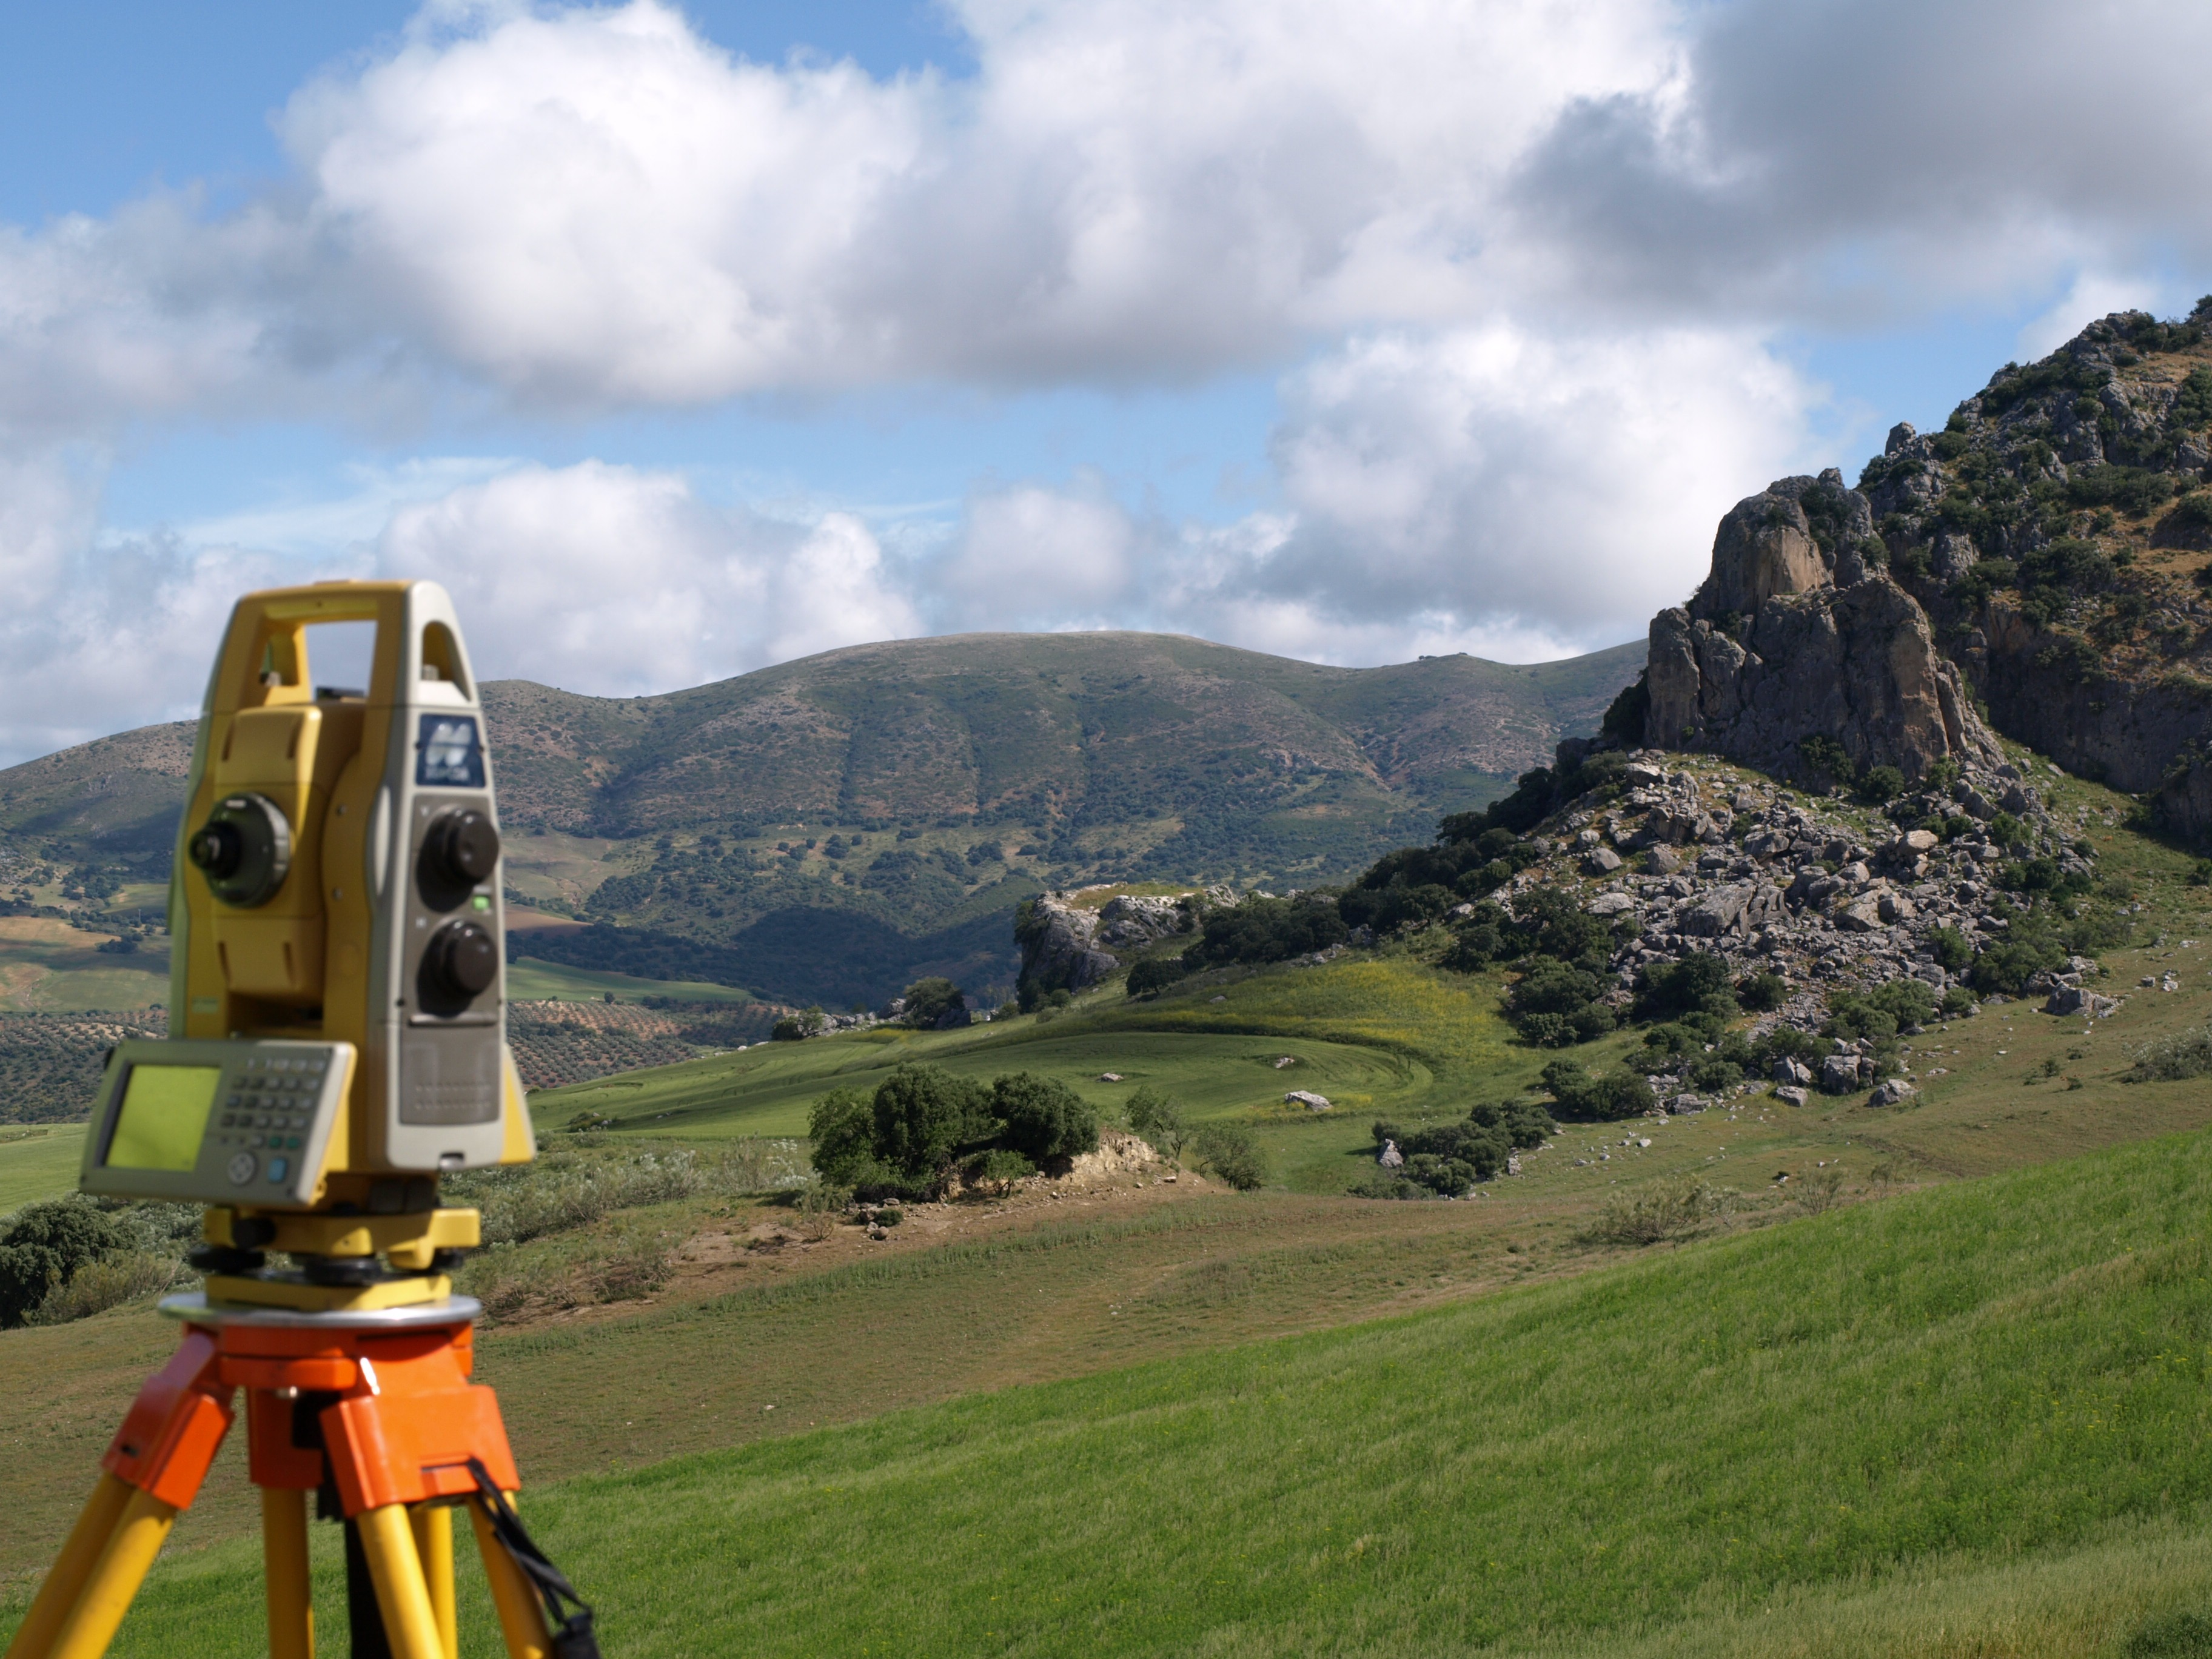
\includegraphics[width=\linewidth]{images/background}
		\end{column}%
		\hfill%
		\begin{column}{.56\textwidth}
			\begin{itemize}
				\item TODO
			\end{itemize}
		\end{column}%
	\end{columns}
	
\end{frame}
% !TeX root = ../presentation.tex

\section{Discussion}
\begin{frame}{Discussion}
	TODO
\end{frame}

\pagebreak
\appendix
\printbibliography

\end{document}
